\chapter{Sequence Learning}
In this chapter we delve into the models used when data is in the form of sequences of variable length. Sequential variable-length data require models that do not make assumptions on the length of the inputs. For example, standard dense linear layers cannot work on variable-length inputs, since the linear layer has a set number of input neurons.

In section~\ref{sec:recurrent_neural_networks} we discuss Recurrent Neural Networks (RNNs), which are sequential models that can be applied to variable-length input data. We cover the most common kind of RNN, the Long Short-Term Memory (LSTM) model, and briefly mention some alternatives.

In section~\ref{sec:sequence_alignments} we discuss how sequential protein data  within a single protein family can be manipulated to avoid the problem of variable-length data altogether, with some other disadvantages as a trade-off.

% Finally, we discuss the transformer model?

\section{Recurrent Neural Networks}
\label{sec:recurrent_neural_networks}
In regular neural networks, we usually think of the input being given to the model, going through a layer which produces an output, which is then fed to the \textit{next} layer of the model. This continues until the data reaches the final layer, which produces the final output.

A recurrent neural network (RNN) is a layer that \textit{recurs} in the model -- for the purposes of RNNs, this refers to the input being processed by the RNN, producing an output, which is then fed into the RNN again, usually in combination with more data. For sequential data, this ``more data'' is usually the next element of the sequence. This enables processing of variable-length data, by making the RNN produce a ``hidden state'' as it processes the sequence. The RNN starts with an initial hidden state, typically initialized to a zero vector. It then takes this hidden state and the first element of the sequence and processes it in some way, to produce the next hidden state. It repeats this process with the new hidden state and the next element of the sequence, until there are no elements in the sequence left. The intermediate hidden states can be thought of as the RNN's ``memory'' about the sequence seen so far. The final hidden state can then be considered the output of the RNN, or one can use the sequence of the intermediate hidden states as an output, depending on the application.

More formally, consider a sequential datapoint $X = (x_1, x_2, \dots, x_n)$. An RNN can be seen as a function $\mathrm{RNN} \colon \prts{\mathbb{R}^h, \mathbb{R}^l} \to \mathbb{R}^h$, where $h$ is the size of the hidden state (a hyperparameter) and $l$ is the size of each $x_i$ of $X$. To apply the RNN on the entire sequence as described above would mean evaluating the following:
\[h_n = \mathrm{RNN}\prts{\mathrm{RNN}\prts{\dots \mathrm{RNN}\prts{\mathrm{RNN}\prts{h_0, x_1}, x_2} \dots, x_{n - 1}}, x_n}\]
Where $h_0$ is the initial hidden state (usually simply $\ve{0}$) and $h_n$ is the final hidden state of the RNN after processing the entire sequence. The $\operatorname{RNN}$ function can be defined in many, many ways, but a few popular options have become commonplace. This includes RNNs like the Long Short-Term Memory (LSTM) or the Gated Recurrent Unit (GRU).

Figure \ref{fig:rnn_comparison} shows a comparison of regular neural networks and RNNs. It also illustrates the concept of ``unrolling'' an RNN. The RNN as shown in figure \ref{subfig:rnn} is a recurrent model, that takes its own output as an input. However, if you unwind the recursion over the entirety of the input sequence, you reach figure \ref{subfig:rnn_unrolled}, which more accurately and explicitly shows how an RNN functions. Note that even though the RNN is drawn multiple times in the unrolled version, it is the same model used again and again.

\begin{figure}[ht]
    \centering
    \begin{subfigure}[t]{0.48\linewidth}
        \centering
        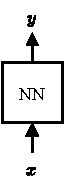
\includegraphics[scale = 1.35]{report/figures/nn.pdf}
        \caption{Regular neural network.}
        \label{subfig:nn}
    \end{subfigure}%
    \hfill
    \begin{subfigure}[t]{0.48\linewidth}
        \centering
        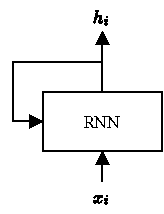
\includegraphics[scale = 1.35]{report/figures/rnn.pdf}
        \caption{Recurrent neural network.}
        \label{subfig:rnn}
    \end{subfigure}
    
    \begin{subfigure}[t]{1\linewidth}
        \centering
        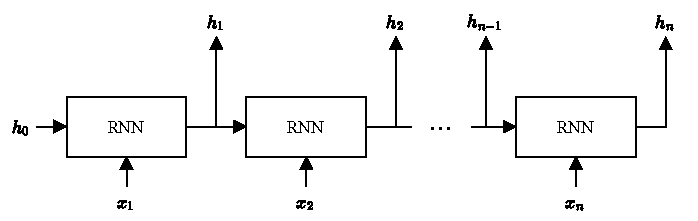
\includegraphics[scale = 1.35]{report/figures/rnn_unrolled.pdf}
        \caption{Unrolled recurrent neural network.}
        \label{subfig:rnn_unrolled}
    \end{subfigure}
    \caption{\subref{subfig:nn}~A regular neural network usually takes a single input and produces a single output. \subref{subfig:rnn}~A recurrent neural network takes a sequence as input, processing each element one at a time, feeding the intermediate hidden states as input to the next recursive call of the RNN. The RNN's output can be considered the last hidden state $\prts{h_n}$ or the entire sequence of hidden states. \subref{subfig:rnn_unrolled}~An ``unrolled'' RNN, more explicitly showing the sequential inputs and the intermediate hidden states.}
    \label{fig:rnn_comparison}
\end{figure}

\subsection{Long Short-Term Memory}
The Long Short-Term Memory (LSTM) is a recurrent neural network (RNN) which uses several \textit{gates} to control how to manipulate the input hidden state based on the input sequence element.

In contrast to some other RNNs, the LSTM actually utilizes two inner states of the same size, where one is known as the ``cell'' state and another is the hidden state. Thus the LSTM can be explained as the function $\mathrm{LSTM} \colon \prts{\prts{\mathbb{R}^h, \mathbb{R}^h}, \mathbb{R}^l} \to \prts{\mathbb{R}^h, \mathbb{R}^h}$ which has the definition \cite{pytorchnn}
\begin{align*}
    \mathrm{LSTM}\prts{\prts{c_{i - 1}, h_{i - 1}}, x_i} &= \prts{c_i, h_i} \\
    c_i &= F_i * c_{i - 1} + I_i * G_t \\
    h_i &= O_i * \tanh\prts{c_i} \\
    F_i &= \mathrm{\sigma}\prts{\mathrm{L_1}\prts{x_i} + \mathrm{L_2}\prts{h_{i - 1}}} \\
    I_i &= \mathrm{\sigma}\prts{\mathrm{L_3}\prts{x_i} + \mathrm{L_4}\prts{h_{i - 1}}} \\
    G_i &= \tanh\prts{\mathrm{L_5}\prts{x_i} + \mathrm{L_6}\prts{h_{i - 1}}} \\
    O_i &= \mathrm{\sigma}\prts{\mathrm{L_7}\prts{x_i} + \mathrm{L_8}\prts{h_{i - 1}}}
\end{align*}
where $O_i$, $G_i$, $F_i$ and $I_i$ are the ``gates'', known as the output gate, cell gate, forget gate and input gate respectively. $\operatorname{\sigma}$ is the sigmoid function while $*$ denotes element-wise multiplication. Each $\mathrm{L_i}$ denotes a linear transformation of the form
\[\mathrm{L_i}\prts{x} = W_i x + b_i\]
where $W_i$ and $b_i$ are learnable parameters of the model, denoted as weight and bias respectively -- thus each $\mathrm{L_i}$ denotes what is otherwise known as a dense linear layer with bias.

The above formal definition is perhaps not the most instructive. Figure \ref{fig:lstm_structure} shows a diagram of the structure of the LSTM. Intuitively, the gates can be understood as operations on the internal ``memory'' of the LSTM (its states). The forget gate $F_i$ can be thought of as deciding what to remove or ``forget'' from the cell state. The input gate $I_i$ and the cell gate $G_i$ then decide what to add to the ``memory'' of the cell state. Finally, the output gate $O_i$ decides how to combine the resulting new cell state $c_i$ and the previous hidden state $h_{i - 1}$ into a new hidden state $h_i$.

\begin{figure}[ht]
    \centering
    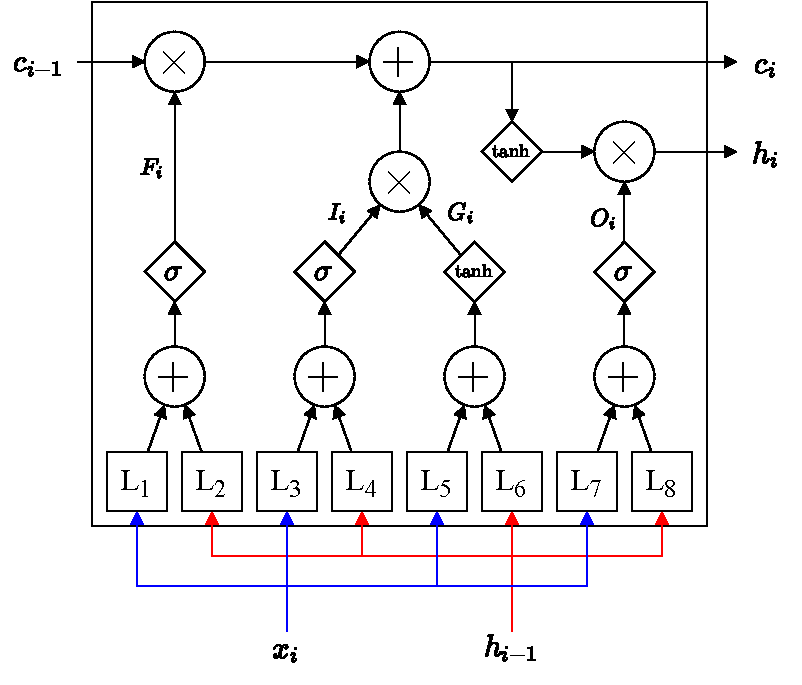
\includegraphics{report/figures/lstm.pdf}
    \caption{The structure of the LSTM, taking $c_{i - 1}$, $h_{i - 1}$ and $x_i$ as inputs, and returning $c_i$ and $h_i$. Squares indicate dense linear layers, diamonds indicate element-wise non-linear activation functions and circles denote binary element-wise operators. Connections from $x_i$ and $h_{i - 1}$ coloured for clarity.}
    \label{fig:lstm_structure}
\end{figure}

The LSTM was designed to avoid the common problem of vanishing gradients in neural networks. This problem is especially prevalent in RNNs, because the repeated application of the RNN leads to a very deep computational graph, in which gradients have to be backpropogated. Due to the depth of this graph, the gradient has a tendency to either vanish or explode. Note how the LSTM actually does not perform a lot of operations on the cell state $c_{i - 1}$. This helps prevent the vanishing gradient problem.

\subsection{Other Recurrent Neural Networks}
There are many other types of RNNs. One of the earliest RNNs was proposed by Jeffrey Elman \cite{elman1990finding}, and consists simply of the following computation \cite{pytorchnn}:
\[\mathrm{Elman}\prts{h_{i - 1}, x_i} = h_i = \tanh\prts{\mathrm{L_1}\prts{h_{i - 1}} + \mathrm{L_2}\prts{x_i}}\]
Where each $\mathrm{L_i}$ again denotes a linear layer, as above.

Another common RNN is the Gated Recurrent Unit (GRU) which, like the LSTM, uses gates to regulate the internal state of the RNN. The GRU however has a somewhat simpler architecture and uses only a single state. The simpler architecture makes the GRU less computationally expensive, and further helps to prevent vanishing or exploding gradients, in comparison to the LSTM. The GRU consists of the following computations \cite{pytorchnn}:
\begin{align*}
    \mathrm{GRU}\prts{h_{i - 1}, x_i} &= h_i \\
    h_i &= z_i * h_{i - 1} + \prts{1 - z_i} * n_i  \\
    z_i &= \mathrm{\sigma}\prts{\mathrm{L_1}\prts{x_i} + \mathrm{L_2}\prts{h_{i - 1}}} \\
    n_i &= \tanh\prts{\mathrm{L_3}\prts{x_i} + r_i * \mathrm{L_4}\prts{h_{i - 1}}} \\
    r_i &= \mathrm{\sigma}\prts{\mathrm{L_5}\prts{x_i} + \mathrm{L_6}\prts{h_{i - 1}}}
\end{align*}
In the above, $r_i$, $z_i$ and $n_i$ are referred to as the \textit{reset}, \textit{update} and \textit{new} gates, respectively. Intuitively, the gates can be thought of a method for the GRU to cleverly interpolate between a newly constructed hidden state $\prts{n_i}$ and the old hidden state. It makes this interpolation using the update gate's result, $z_i$. The reset gate roughly decides what to keep/forget from the old hidden state when constructing the new one.

There are many more RNNs, of which many are variations of the above. For example, the multiplicative LSTM (mLSTM) \cite{krause2016multiplicative} extracts certain information from the previous hidden state, which it then uses in the LSTMs gates, instead of the previous hidden state. That is, it calculates
\[m_i = \mathrm{L_{m_1}}\prts{x_i} * \mathrm{L_{m_2}}\prts{h_{i - 1}}\]
and then uses $m_i$ instead of $h_{i - 1}$ in the gates of the LSTM.

\section{Sequence Alignments}
\label{sec:sequence_alignments}
As proteins are sequential in nature, RNNs can be used to integrate them into deep learning models. However, despite RNNs being suited for sequential data, it is not always the best model to use for proteins. While RNNs are able to process proteins, there are certain disadvantages in the way that RNNs do this. For example, when an RNN processes a single amino acid, it cannot take into account any remaining amino acids of the protein, because the RNN hasn't reached those amino acids yet. Also, the RNN cannot even directly take into account the previous amino acids -- it can only use the hidden state up to a certain point.

\subsection{Dense models}
